% !TeX spellcheck = cs_CZ
%{\tikzset{external/prefix={tikz/FYZI/}}
% \tikzset{external/figure name/.add={ch41_}{}}
%=========================== Kapitola: Brownův pohyb ==============================================
\setchaptertoc
\chapter{Brownův pohyb}\label{fyz:IchapXLI}

  \section{Ekvipartičnost energie}\label{fyz:IchapXLIsecI}
  \section{Tepelná rovnováha záření}\label{fyz:IchapXLIsecII}
  \section{Ekvipartičnost a kvantový oscilátor}\label{fyz:IchapXLIsecIII}
  \section{Náhodná procházka}\label{fyz:IchapXLIsecIV}
  \section{Příklady a cvičení}\label{fyz:IchapXLIsecV}

  \begin{figure}[hb!] %\ref{fyz:fig0483}
    \centering
    \subcaptionbox{\label{fyz:fig0483a}}{\luafigure[0.7]{fyz_fig0483a.pdf}}  \\
    \subcaptionbox{\label{fyz:fig0483b}}{\luafigure[0.6]{fyz_fig0483b.pdf}}  
    \caption{
             (\cite[s.~601]{Feynman01}).}
    \label{fyz:fig0483}
  \end{figure}

  \begin{figure}[hb!] %\ref{fyz:fig0484}
    \centering
    \subcaptionbox{\label{fyz:fig0484a}}{\luafigure[0.4]{fyz_fig0484a.pdf}}
    \subcaptionbox{\label{fyz:fig0484b}}{\luafigure[0.4]{fyz_fig0484b.pdf}}
    \caption{
             (\cite[s.~601]{Feynman01}).}
    \label{fyz:fig0484}
  \end{figure}

    \begin{figure}[ht!] %\ref{fyz:fig0485}
      \centering
      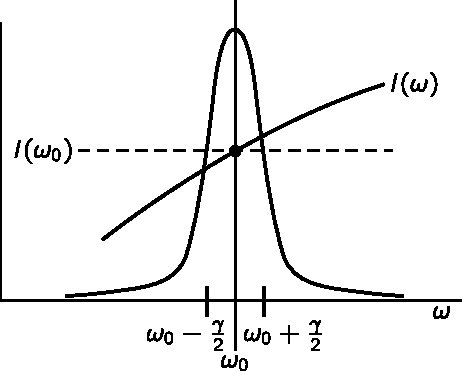
\includegraphics[width=0.7\linewidth]{fyz_fig0485.pdf}
      \caption{ 
               (\cite[s.~707]{Feynman01})}
      \label{fyz:fig0485}
    \end{figure}

    \begin{figure}[ht!] %\ref{fyz:fig0486}
      \centering
      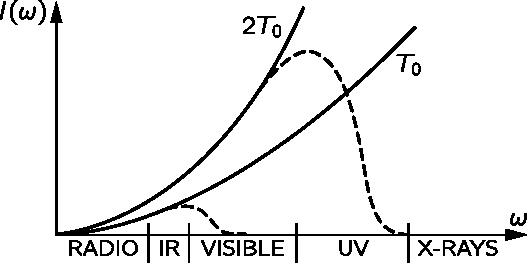
\includegraphics[width=0.7\linewidth]{fyz_fig0486.pdf}
      \caption{ 
               (\cite[s.~707]{Feynman01})}
      \label{fyz:fig0486}
    \end{figure}

    \begin{figure}[ht!] %\ref{fyz:fig0487}
      \centering
      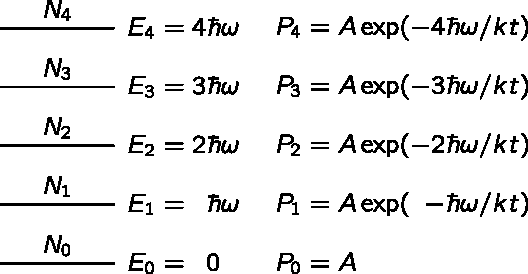
\includegraphics[width=0.7\linewidth]{fyz_fig0487.pdf}
      \caption{ 
               (\cite[s.~707]{Feynman01})}
      \label{fyz:fig0487}
    \end{figure}

    \begin{figure}[ht!] %\ref{fyz:fig0488}
      \centering
      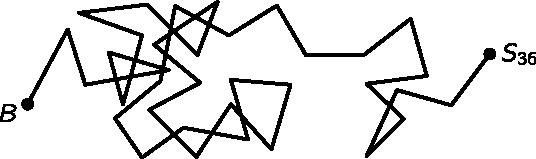
\includegraphics[width=0.7\linewidth]{fyz_fig0488.pdf}
      \caption{ 
               (\cite[s.~707]{Feynman01})}
      \label{fyz:fig0488}
    \end{figure}
    
    \todo[inline]{Kapitola fey1ch41 je zcela prázdná, pouze obrázky}     
%} %tikzset
%---------------------------------------------------------------------------------------------------